\chapter{Bayesian learning for DPPs}

So far we have seen two different estimation techniques for the parameters of DPPs. Although we proved that they provide reasonable estimators in the sense that they are consistent, they have some drawbacks. For example we have seen that the MLEs for the different parameters do not exist in general, let alone that they are impossible to compute in reality. Further
%Firstly, we saw that the maximum likelihood estimator does not exist in general and in some cases one needs a fairly high amount of samples to ensure that it does. Secondly 
all of the estimators presented so far are point estimators, i.e. they return a single value for the desired parameter. Obviously this does not allow to capture any uncertainties and we have already seen in \todo{cite} that the selection of the most possible outcome -- in this case the MLE -- might not yield a very typical one for a given random variable.
Those are some reasons to consider the Bayesian approach of parameter estimation where the goal is to give a distribution -- called the posterior -- of the parameter that should be estimated instead of a single value. This can also help to overcome some -- maybe even all of the problems presented above.

At first we will present the general idea of Bayesian parameter estimation and then we will turn towards the question of computability. %Since the normalisation constant of the 
For this we will follow the approach of \cite{affandi2014learning} and turn towards the popular Markov chain Monte Carlo (MCMC) methods and quickly explain their philosophy and how they can be used to approximate the posterior distribution of the parameter that is to be estimated.

\section{Bayesian approach to parameter estimation}

For the introduction of the general Bayesian setup we pursue like in \cite{rice2006mathematical}. We are -- just like in the case of MLE -- in the setting that we want to estimate a parameter \(\theta\in\Theta\) based on some relisations \(x = (x_1, \dots, x_n)\) of some random variables \(X = (X_1, \dots, X_n)\) where we have given a family
\[\mathcal F = \Big\{ f_{X| \Theta}(\cdot |\theta) \mid \theta\in\Theta\Big\}\]
of densities with respect to \(\mu^n\coloneqq\prod_{i=1}^n\mu(\mathrm d x_i)\). This time however we are not interested in returning a single value \(\theta\) because this would be a vast simplification of the stochastic nature of the estimator. Thus we want to obtain a probability distribution over whole \(\Theta\) that indicates how the parameters are to have caused the observed data. In order to present the procedure we will introduce the frame we will work in.

\begin{emp}[Setting]
Let \(\Theta\) be a measurable space and \(\nu\) be a measure on \(\Theta\). Further let \(f_\Theta\colon \Theta\to[0, \infty]\) be a probability density with respect to \(\nu\), i.e.
\[\int f_\Theta(\theta)\nu(\mathrm{d}\theta) = 1\]
which we will call the \emph{prior} distribution of the parameter \(\theta\).
\end{emp}

Usually the prior distribution will encode some perceptions we have of the parameter. For example if we are trying to estimate a physical constant that we know has to be positive, then it is reasonable to select a prior that has its whole mass on the positive real line. However there is no clear set of rules how one can select a suitable prior to a given problem. %Further we will see how the prior gives a way of regularisation in the sense that 

%To obtain the distribution of \(\theta\) given the observations \(x\) we will first construct the joint density of both parameters and then take the marginal distribution of \(\theta\).
The density \(f(x|\theta)\) describes how likely the observations are under the parameter theta and we want to find an expression of how likely the parameter theta is under the observations \(x\). %and \(f(\theta)\) 
In order to obtain this, we will work with the joint density
\[f_{X, \Theta}(x, \theta) = f_{X|\Theta}(x|\theta) f_\Theta(\theta) \quad \text{with respect to } \mu^n \times \nu \]
and condition this onto \(x\). This yields
\begin{equation}\label{post}
\begin{split}
f_{\Theta| X}(\theta|x) = \frac{f_{X, \Theta}(x, \theta)}{\int f_{X, \Theta}(x, \theta)\nu(\mathrm{d}\theta)} = \frac{f_{X|\Theta}(x| \theta) f_\Theta(\theta)}{\int f_{X, \Theta}(x, \theta)\nu(\mathrm{d}\theta)}
\end{split}
\end{equation}

\begin{defi}[Posterior distribution]
The density \(f_{\Theta|X}\) is called the \emph{posterior distribution} of the parameter \(\theta\) given the data \(x\).
\end{defi}

%From now on we will assume -- just like in the case of MLE -- that our observations are independent and identically distributed and hence their joint distribution factorises and we obtain
%\[f_{\Theta| X}(\theta|x) \propto f_\Theta(\theta) \prod_{i=1}^n f_{X|\Theta}(x_i| \theta)\]

This posterior density is already the object we are interested in which is supposed to give us the information of the distribution of the parameter given the data \(x\). It is proportional to the likelihood \(f_{X|\Theta}(x|\theta)\) of the occuring data times the prior \(f_\Theta(\theta)\) which can be understood in the way, that 

\begin{emp}[Comparison to MLE]
Maybe one feels slightly uncomfortable with the need of a choice for the prior distribution and it turns out that this is in fact a difficult step that has to be taken with a certain amount of care. However we could pretend for one moment to be completely ignorant in the sense that we do not know anything about the parameter and hence we don�t feel in the position to propose a reasonable prior. Then we could simply choose the uniform distribution as a prior -- given it exists -- and would obtain
\[f_{\Theta| X}(\theta|x) \propto f_{X|\Theta}(x|\theta). \]
Hence we can regain the MLE from our posterior distribution since it is just the mode, i.e. the maximiser of the posterior density. This relation to the MLE can be seen in Figure \ref{fig:3.1}. Hence the Bayesian approach is a a more powerful tool than MLE and allows also to capture the random uncertainty of the parameter \(\theta\) and we have seen that the mode is  not always a vey typical outcome of a random variable\todo{cite}.
\begin{figure}[h!]
	\centering
	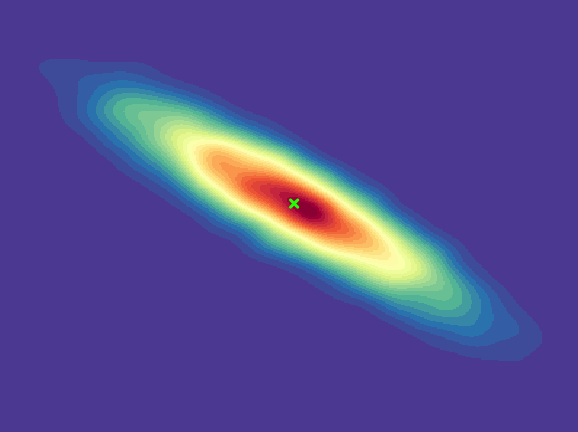
\includegraphics[width=0.6\textwidth]{heatmap-log-linearity-SliceSampling-new-3}
%	\tag{1}
	\caption{Approximated posterior density of the two dimensional log linearity constant of a two dimensional DPP with a uniform distribution as a prior. The MLE estimator is marked green and is at the mode of the distribution.}
	\label{fig:3.1}
\end{figure}

A second advantage over the MLE presented in the third chapter is, that it might be possible to computationally approximate the posterior density but not the MLE. This is typically the case if the log likelihood function is not concave, like in the setting of the MLE of the whole elementary kernel \(L\). In fact only hard step in the calculation of the posterior \eqref{post} is the computation of the normalisation constant
\[\int f_{X,\Theta}(x, \theta) \nu(\mathrm{d}\theta). \]
This step can actually also not be performed efficiently for the case of the estimation of \(L\), however we will introduce the methods of Markov chain Monte Carlo simulation that allow an approximation of the posterior without the need to compute the normalisation contant.
\end{emp}

\begin{emp}[Regularisation through the prior]

\end{emp}

%\begin{enumerate}
%\item explain general procedure and say something about intuition
%\item explain the benefits, namely:
%\begin{enumerate}
% \item can capture uncertainty
% \item might me more feasible
% \item is an extension, at least if there is a uniform distribution on the parameter space
%\item offers a method for regularisation, i.e. will sometimes work if MLE doesn�t (properly) work due to statistical fluctuations like overfitting of noise
%\end{enumerate}
%\item 
%\end{enumerate}

\subsubsection*{Expression of the posterior for DPPs}

Now we will express the posterior in the case of DPPs under the following conditions.

\begin{emp}[Setting]
Let \(\Theta\) be a set and \(L(\theta)\in\mathbb R^{N\times N}_{\text{sym}, +}\) be an elementary kernel. Further we assume that we have independent realisations \(A_1, \dots, A_n\) of a  \(L\)-ensemble.
\end{emp}

Typically the parametrisations \(\theta\mapsto L(\theta)\) will be one of the three parametric models in III.2.1, i.e. \(\theta\) will either be the whole kernel itself, the quality vector, or the log linearity constant of the qualities and \(L(\theta)\) the associated elementary kernel.

The independence relation leads to a factorisation of the density and we obtain the following expression for the posterior density
\begin{equation}\label{post2}
f(\theta|A_1, \dots, A_n) \propto f_\Theta(\theta) \prod_{i=1}^n f(A_i|\theta) = f_\Theta(\theta) \prod_{i=1}^n \frac{\det(L(\theta)_{A_i})}{\det(L(\theta) + I)}
\end{equation}
where we dropped some indices of the density functions in slight abuse of notation.

Unfortunately the normalisation constant
\begin{equation}\label{norma}
\int f(\theta|A_1, \dots, A_n)\nu(\mathrm{d}\theta) = \int f_\Theta(\theta) \prod_{i=1}^n \frac{\det(L(\theta)_{A_i})}{\det(L(\theta) + I)}\nu(\mathrm{d}\theta)
\end{equation}
can neither be computed analytically nor numerically in an efficient way. This problem can be solved through the powerful method of Markov chain Monte Carlo simulation that allow to approximate a distribution with only the knowledge of its unnormalised density.

\section{Markov chain Monte Carlo methods}

The method of of Markov chain Monte Carlo (MCMC) simulation arose almost as early as the one Monte Carlo\footnote{A legend has it that the name Monte Carlo was given to the work of von Neumann and Ulam %in Los Alamos 
by a colleage referring to Ulam�s uncle who lost a significant amount of money gambling in the Monte Carlo casino in Monaco.} simulation itself and since then a rich theory and a broad range of applications have been found. However we can only give a short overview over the basic principles and refer to \cite{meyn2012markov} for an introduction of Markov chain theory and to \cite{robert2013monte} for a survey on (Markov chain) Monte Carlo methods.

We motivated MCMC methods for the approximation of the distribution \(\pi\) under the knowledge of its unnormalised density. In the nutshell the idea is to construct an ergodic Markov chain \((X_n)_{n\in\mathbb N}\) with stationary distribution \(\pi\), i.e. such that one has
\[ \hat{\mathbb P}_n =\frac1n \sum_{i=1}^n \delta_{X_n} \xlongrightarrow{n\to\infty} \pi. \]
This Markov chain can then be simulated using Monte Carlo methods. However to explain this in more detail we need to recapture some notions of Markov chains.

% The reason nables amongst other things to sample from or to approximate a distribution without knowing the normalisation constant.

\subsection{Reminder on Markov chains}

We will provide an extremely short presentation of onyl the results that we will use to explain the core of MCMC methods. However this will not contain any proofs and hence it can not replace the study of the already mentioned text books. However let in the following \((\mathcal X, \mathcal B(\mathcal X))\) be a measurable space.


\begin{defi}[Markov chain]
\begin{enumerate}
\item A \emph{transition kernel} is a function \[K\colon\mathcal X\times\mathcal B(\mathcal X)\to[0, 1]\] such that
\begin{enumerate}
\item \(K(x, \cdot)\) is a probability measure for every \(x\in\mathcal X\) and
\item \(K(\cdot, A)\) is measurable for every \(A\in\mathcal B(\mathcal X)\).
\end{enumerate}
\item A \emph{Markov chain} with values in \(\mathcal X\) is a collection \((X_n)_{n\in\mathbb N}\) of \(\mathcal X\) valued random variables such that
\[\mathbb P\big(X_0\in A_0, \dots, X_n\in A_n\big) = \int_{A_0} \gamma(\mathrm{d}x_0) \int_{A_1} K(x_0, \mathrm{d}x_1) \cdots \int_{A_n} K(x_{n-1}, \mathrm{d}x_n) \]
for all \(A_1, \dots, A_n\in\mathcal B(\mathcal X)\) where \(\gamma\) denotes the distribution of \(X_0\).
\end{enumerate}
\end{defi}

We will call \(\gamma\) the \emph{initial} or \emph{starting distribution} of the Markov chain and will denote the distribution of this Markov chain by \(\mathbb P_\gamma\) and the expectation with respect to it by \(\mathbb E[\cdot]\). Further one can show that there is a Markov chain for any given %we note that we obtain a Markov chain with
transition kernel \(K\) and initial distribution \(\gamma\)\todo{cite}. %by taking \(X_0\) distributed according to \(\gamma\) and \(X_{n+1}\) distributed according to \(K(X_n, \cdot)\) for \(n = 0, 1, \dots\).
 If the initial distribution is deterministic, i.e. \(\gamma = \delta_x\) for one \(x\in\mathcal X\), then we also write \(\mathbb P_x\) for the distribution of the Markov chain.

We close this paragraph by introducing the notation
\[K^n(x, A) \coloneqq \mathbb P_x(X_n\in A). \]

%\begin{enumerate}
% \item Definition
%\item irreducibility
% \item existence of stationary distributions
%\item reversibility
%\item detail-balance
%\item Ergodicity 
%\item idea of MCMC
%\end{enumerate}

\subsubsection*{Irreducibility, recurrence and existence of stationary distributions}

From now on we will fix a reference measure \(\mu\) on \(\mathcal X\).

\begin{defi}[Irreducibility and recurrence]
\begin{enumerate}
\item We say a Markov chain is \emph{\(\mu\) irreducible} if for every \(A\in\mathcal B(\mathcal X)\) with \(\mu(A)>0\) there is an index \(n\in\mathbb N\) such that
\[\mathbb P_x(X_n\in A) = K^n(x, A) > 0 \quad \text{for all } x\in\mathcal X. \]
\item A Markov chain \((X_n)_{n \in\mathbb N}\) is called \emph{recurrent} if
\begin{enumerate}
\item there is a measure \(\mu\) on \(\mathcal B(\mathcal X)\) such that \((X_n)\) is \(\mu\)-irreducible and
\item if for every \(A\in\mathcal B(\mathcal X)\) with \(\mu(A)>0\) the expected number of visits of \(A\) is infinite, i.e.
\[\mathbb E_x\left[\left\lvert \left\{ n\in\mathbb N \mid X_n\in A\right\} \right\rvert\right] = \infty \quad \text{for every } x\in A.\]
\end{enumerate}
\item A Markov chain is called \emph{Harris recurrent} if it is recurrent and the number of visits is almost surely infinite, i.e. for any \(A\in\mathcal B(\mathcal X)\) with \(\mu(A)>0\) we have
\[\mathbb P_x\left(\left\lvert \left\{ n\in\mathbb N \mid X_n\in A\right\} \right\rvert = \infty\right) = 1 \quad \text{for every } x\in A.\]
\end{enumerate}
\end{defi}

\begin{defi}[Stationary distributions]
Let \(\pi\) be a measure on \(\mathcal B(\mathcal X)\). We call \(\pi\) an \emph{invariant} or \emph{stationary distribution} of a Markov chain with kernel \(K\), if \(X_{n+1}\) is distributed according to \(\pi\) whenever \(X_n\) is distributed according to \(\pi\). This is equivalent to
\[\pi(A) = \int K(x, A)\pi(\mathrm d x) \quad \text{for all } A\in\mathcal B(\mathcal X). \]
\end{defi}

\begin{theo}[Existence of stationary distributions]
If \((X_n)_{n\in\mathbb N}\) is a recurrent Markov chain, there exists an invariant \(\sigma\)-finite measure which is unique up to a multiplicative factor.
\end{theo}

\subsubsection*{Convergence to the stationary distribution and ergodicity}

We will not introduce the notion of periodic and aperiodic Markov chains here, because it would distract us from our actual goal. However we still present the following result that only holds for aperiodic Markov chains and refer to \cite{meyn2012markov} for further information. The reason why we still present the theorem is that it explains how one can approximately sample from the stationary distribution of a Markov chain, namely it says that the distribution of \(X_n\) converges to the invariant distribution.

\begin{theo}[Convergence to stationary distribution]
Let \((X_n)_{n\in\mathbb N}\) be a Harris recurrent and aperiodic Markov chain with stationary distribution \(\pi\). Let further \(\gamma_n\) be the distribution of \(X_n\), then we have
\[\left\lVert \gamma_n - \pi \right\rVert_{TV} \xlongrightarrow{n\to\infty} 0 \]
monotone. Here \(\left\lVert \cdot \right\rVert_{TV}\) denotes the total variation of a measure
\[\left\lVert \mu \right\rVert_{TV}\coloneqq \sup_{\mathcal E}\sum\limits_{E\in\mathcal E} \left\lvert \mu(E) \right\rvert\]
where the supremum is taken over all finite families of disjoint measurable sets.
\end{theo}

\begin{theo}[Ergodic theorem]
Let \((X_n)_{n\in\mathbb N}\) be a Harris recurrent Markov chain with \(\sigma\)-finite stationary distribution \(\pi\), then \((X_n)_{n\in\mathbb N}\) is \emph{ergodic}. This means that if %\(\gamma_n\) be the distribution of \(X_n\), then we have
\[\hat{\mathbb P}_n \coloneqq \frac1n \sum_{i=1}^n \delta_{X_i} \]
is the empirical measure, we have almost surely have
\begin{equation}\label{ergo}
\int f(x) \hat{\mathbb P}_n(\mathrm dx) \xlongrightarrow{n\to\infty} \int f(x)\pi(\mathrm dx)
\end{equation}
for every \(\pi\) integrable function \(f\).
\end{theo}

In the particular case that \(\mathcal X\) is a topological space and \(\mathcal B(\mathcal X)\) is the Borel algebra and if \(\pi\) is a finite measure, we obtain the almost surely weak convergence of \(\hat{\mathbb P}_n\) towards \(\pi\). This means that the convergence in \eqref{ergo} almost surely holds
%\[\int f(x) \hat{\mathbb P}_n(\mathrm dx) \xlongrightarrow{n\to\infty} \int f(x)\pi(\mathrm dx)\]
for all continuous and bounded functions \(f\). This means that \(\hat{\mathbb P}_n\) are approximations of the invariant distribution in the sense of weak convergence, which is metrisable\todo{cite}.


\subsubsection*{Idea of Markov chain Monte Carlo methods}

The motivation of the study of Markov chain Monte Carlo methods was to approximate the posterior distribution \eqref{post2}. The idea is now to construct and then simulate a Markov chain \((X_n)_{n\in\mathbb N}\) such that the empirical measures \(\hat{\mathbb P}_n\) converge to the posterior. In order to achieve this we only have to check the requirements of the ergodic theorem. This means we want to construct a Harris recurrent Markov chain with the posterior density as an invariant distribution without having to compute the normalisation constant \eqref{norma}.

\begin{defi}[MCMC methods]
A Markov chain Monte Carlo (MCMC) method for the simulation of a distribution \(\pi\) is any method that produces an ergodic Markov chain \((X_n)_{n\in\mathbb N}\) whose stationary distribution is \(\pi\).
\end{defi}

We will present the two most common MCMC methods which are the Metropolis-Hastings random walk and the method of slice sampling.

\subsection{Metropolis-Hastings random walk}

The Metropolis-Hastings random walk is maybe the most wide spread MCMC method and certainly one of the oldest. It was actually proposed in the early 1950s from researchers of the American nuclear programme in Los Alamos (c.f. \cite{metropolis1953equation}). First we will touch on the theoretical aspects -- mostly the ergodicity -- of the MH random walk and follow the ideas present in \cite{robert2013monte}.

%The idea of the Metropolis-Hastings (MH) random walk was introduced as early as 1953 by Metropolis (c.f. \cite{metropolis1953equation}) and later adapted by Hastings in \
{hastings1970monte}.

\begin{emp}[Setting]
Let \(\Theta\) be a measurable space, \(\mu\) a measure on that space and \(f\colon\mathcal X\to[0, \infty]\) a function with finite integral
\[Z = \int f(x) \mu(\mathrm{d}x)\in(0, \infty).\]
Our goal is to find a Harris recurrent Markov chain with invariant distribution
\[\pi(A)\coloneqq \frac1Z \int_A f(x)\mu(\mathrm dx). \]
Let further
\[\left\{ f(\cdot|x) \mid x \in\mathcal X\right\}\]
be a family of probability distributions, which we call the \emph{proposal distributions}.
\end{emp}

\begin{emp}[The MH random walk]
Given the first \(n\) states of the Markov \(X_1= x_1, \dots, X_n = x_n\), we define \(X_{n+1}\) as follows. Let \(Y\) be distributed according to \(f(\cdot|x_n)\mathrm d\mu\) and take one realisation \(y\) of \(Y\). Then set
\[X_{n+1}\coloneqq\begin{cases}\; y \quad & \text{with probability } \rho(x_n, y) \\\; x_n & \text{with probability } 1 - \rho(x_n, y) \end{cases} \]
where
\[\rho(x, y) \coloneqq \min\left\{ \frac{f(y) f(x|y)}{f(x)f(y|x)}, 1\right\}.\]
\todo{say something about dividing by zero}
The first step of the random walk, namely the sampling of \(y\) is called the \emph{proposal step} and the second one the \emph{accept-reject step}. The MH random walk can be expressed in pseudo code.
\begin{algorithm}
\caption{A single step of the MH random walk \label{alg:MH}}
\begin{algorithmic}[1]
\Require{First \(n\) samples \(x_1, \dots, x_n\)}
\State \(y\sim f(\cdot|x_n)\mathrm d\mu\)
\State \(a\sim \mathcal U([0, 1])\)
\If{\(a\le \rho(x_n, y)\)}
  \State \(x_{n+1}\gets y\)
\EndIf
\State\Return{\(x_{n+1}\)}
\end{algorithmic}
\end{algorithm}
\end{emp}

%To the readers familiar with Markov chain theory, it will be immediately clear that \((X_n)_{n\in\mathbb N}\) is a Markov chain, since \(X_{n+1}\) can be written as a function of \(X_n\) and a stochastic influence. 
To see that the definition above indeed yields a Markov chain we convince ourselves that the transition kernel is given by
\[K(x, A) = \int_A\rho(x, y)f(y|x) \mu(\mathrm dy) + (1 - m(x)) \delta_x(A) %\int_A
\]
where \(\delta_x\) is the Dirac measure in \(x\) and
\[m(x) = \int \rho(x, y) f(y|x) \mu(\mathrm dy) \]
is the acceptance rate\todo{is this true?}.

\begin{prop}[Stationary distribution]
\todo{under which support conditions?}
%Let \((X_n)_{n\in\mathbb N}\) be the Metropolis-Hastings random walk. Then
The probability measure \(\pi\) is a stationary distribution of MH random walk.
\end{prop}
\begin{proof}
We have
\begin{equation}\label{calc1}
\begin{split}
\int K(x, A) \pi(\mathrm dx) & =  \frac1Z \int\left( \int_A \rho(x, y) f(y|x) \mu(\mathrm dy) + (1 - m(x)) \delta_x(A)\right) f(x) \mu(\mathrm dx) %\\
%& = 
\end{split}
\end{equation}
We note that
\[\rho(x, y) f(y|x) f(x) = \rho(y, x) f(x|y) f(y)\]
and obtain
%Using the definition of \(m(x)\) we obtain
for the second term
\begin{equation*}
\begin{split}
\frac1Z \int m(x) \delta_x(A) f(x) \mu(\mathrm dx) & = \frac1Z\int\int \rho(x, y) f(y|x) \mu(\mathrm dy) \delta_x(A) f(x) \mu(\mathrm dx) \\
 & = \frac1Z\int_A \int \rho(x, y) f(y|x)f(x) \mu(\mathrm dy) \mu(\mathrm dx) \\
 & = \frac1Z\int \int_A \rho(x, y) f(y|x)f(x) \mu(\mathrm dx) \mu(\mathrm dy) \\
 & = \frac1Z\int \int_A \rho(y, x) f(x|y) \mu(\mathrm dx) f(y) \mu(\mathrm dy)
\end{split}
\end{equation*}
where we used Fubini-Tonelli theorem\footnote{The Fubini-Tonelli theorem states that the order of integration with respect to two \(\sigma\)-additive measures can be swapped, if the integrated function is non negative.} in the second to last step. We note that now two of the terms in \eqref{calc1} cancel out and we obtain
\[\int K(x, A) \pi(\mathrm dx) = \frac1Z \delta_x(A) f(x) \mu(\mathrm dx) = \pi(A). \]
\end{proof}

Now we are aiming to prove that the MH random walk is Harris recurrent because then the ergodic theorem yields that the empirical measures associated with the Markov chain will actually converge to \(\pi\). Obviously this is not for all proposal families in general the case, for example we could consider that the proposal distribution \(f(\cdot|x)\) is just the Dirac measures in \(x\)\footnote{Obviously this is slightly formal, because the Dirac measure can typically not be expressed through a density. However rigorous examples can be constructed similarly.}. Then the MH random walk would never leave its initial position which will typically be a deterministic point. Hence the empirical measures only be the Dirac measure in the starting point and hence not converge towards \(\pi\).

The first step towards Harris recurrence is to show irreducibility and this will already give us some hints what families of proposal are sensible.
% and the first step for this is the irreducibility.

\begin{prop}[Irreducibility]
Assume that the proposal family is strictly positive, i.e.
\[f(y|x) > 0 \quad \text{for all } x, y\in\mathcal X. \]
Then the MH random walk is \(\pi\) irreducible.
\end{prop}
\begin{proof}
For any measurable set \(A\subseteq\mathcal X\) with positive measure \(\pi(A)>0\) we have
\[K(x, A) \ge \int_A \rho(x, y)f(y|x) \mu(\mathrm d y) > %= \int_A \min\left\{ \frac{f(y) f(x|y)}{f(x)f(y|x)}, 1\right\}f(y|x) \mu(\mathrm d y) > 
0. \]
To see this, we can assume that this would not hold, but then the integrant has to zero \(\mu\) almost surely. Since \(f(y|x)\) is strictly positive this would imply \(\rho(x, y) = 0\) and hence \(f(y) = 0\) almost surely with respect to \(\mu\). However this is a contradiction to
\[\pi(A) = \int_A f(y)\mu(\mathrm dy) > 0.\]
\end{proof}

%\begin{prop}[Harris reccurence]
%If the MH random walk is \(\pi\) irreducible, then it is also Harris recurrent.
%\end{prop}
%\begin{proof}
%We refer to Lemma 7.3 in \cite{robert2013monte}.
%\end{proof}

Now we can formulate the ergodicity for \(\pi\) irreducible MH random walks.

\begin{theo}[Ergodicity of the MH random walk]
If the MH random walk is \(\pi\) irreducible, then it is also Harris recurrent and hence ergodic.
\end{theo}
\begin{proof}
We refer to Lemma 7.3 in \cite{robert2013monte} for the proof of Harris recurrency, the ergodicity then follows from the ergodic theorem.
\end{proof}

\subsubsection*{Implementation of the MH random walk}

So far we have presented the theoretical foundations of the MH random walk and now we want to touch on a few aspect of the simulation process. For this part we shall point the reader towards the very gentle introduction \cite{robert1999metropolis} to the implementation of the MH random walk which also provides coding examples.

\begin{emp}[Choosing a proposal family]

\end{emp}

\begin{emp}[Tuning the proposal]

\end{emp}

\subsection{Slice sampling}

Slice sampling is a different MCMC method and quite similar to the MH random walk. Nevertheless it has the theoretical benefit that one does not have to define a family of proposal distributions and that the constructed Markov chain is always irreducible. However we will see that at least when one wants to simulate the slice sampling one runs into similar problems. We begin by fixing our frame we will work in. %  where one has to model 

\begin{emp}[Setting]
Let \(\Theta\) be a measurable space, \(\mu\) a measure on that space and \(f\colon\mathcal X\to[0, \infty]\) a function with finite integral
\[Z = \int f(x) \mu(\mathrm{d}x)\in(0, \infty).\]
In particular there is \(\hat x\in\mathcal X\) such that \(f(\hat x)>0\). Our goal is to find a Harris recurrent Markov chain with invariant distribution
\[\pi(A)\coloneqq \frac1Z \int_A f(x)\mu(\mathrm dx). \]
Further we will assume -- maybe after modification of \(f\) on a \(\mu\) Null set -- that 
\[f\le \left\lVert f \right\rVert_{L^\infty(\mu)} = \inf \Big\{ \alpha\in\mathbb R \mid f \le \alpha \text{ almost surely with respect to } \mu \Big\}. \]
\end{emp}

\begin{emp}[Definition of the Markov chain]
Assume we have already given the first \(n\) samples \(x_1, \dots, x_n\) of the Markov chain. If we have \(f(x_n)=0\), then we set \(x_{n+1}\coloneqq \hat x\). Otherwise we sample \(y\) according to the uniform distribution on \([0, f(x_n)]\) and define the \emph{slice}
\[S\coloneqq S(y)\coloneqq \left\{ x\in\mathcal X \mid f(x) \ge y \right\}. \]
Note that because \(y \le f(x_n)\le \left\lVert f \right\rVert_{L^\infty(\mu)}\) we have \(\mu(S)>0\) as well as
\[ \mu(S) \le y^{-1} \int_S f(x)\mu(\mathrm dx)<\infty \]
where we used Markov�s inequality as well as \(y>0\) almost surely. Now draw \(x_{n+1}\) according to the uniform distribution on \(S\). Note that \(f(x_n)>0\), then \(f(x_{n+1})\ge y > 0\) almost surely.

In pseudo code the algorithm takes the following form.
\begin{algorithm}
\caption{A single slice sampling step \label{alg:slice-sampling}}
\begin{algorithmic}[1]
\Require{First \(n\) samples \(x_1, \dots, x_n\)}
 \If \(f(x_n) = 0\)
  \State \(x_{n+1}\gets \hat x\)
\Else
  \State \(y\sim \mathcal U([0, f(x_n)])\)
  \State \(S\gets \left\{ x\in\mathcal X \mid f(x) \ge y \right\}\)
  \State \(x_{n+1} \sim \mathcal U(S)\)
\EndIf
\State\Return{\(x_{n+1}\)}
\end{algorithmic}
\end{algorithm}
\end{emp}
\todo{maybe add a picture?}

%\Require{First \(n\) samples \(x_1, \dots, x_n\)}
%\If{\(f(x_n) = 0\)}
%  \State \(x_{n+1}\gets x_0\)
  %\Break
%\Else
%  \State \(y\sim \mathcal U([0, f(x_n)])\)
%  \State \(S\gets \left\{ x\in\mathcal X \mid f(x) \ge y \right\}\)
%  \State \(x_{n+1} \sim \mathcal U(S)\)

The reason why we have to take of the case \(f(x_n)=0\) individually is, that there typically is no uniform distribution on the slice \(S(0)\).

If we compare the Markov chain to the MH random walk, we noticr that in the slice sampling we first create a random threshold \(y\) and then sample uniformly from all points that satisfy this threshold. This is just the other way round than in the MH random walk where we first make a proposal for the next state of the Markov chain and then decide whether we will accept it or not.

Just like in the case of the MH random walk we can explicitly give the transition kernel and use this expression then to check that \(\pi\) is a stationary distribution. The kernel of the Markov chain that arises from the slice sampling iteration is given by
\[K(x, A) = \int_\mathbb R\frac{\mathds{1}_{[0, f(x)]}(y)}{f(x)} \cdot Z(y)^{-1} \int_A \mathds{1}_{[y, \infty)}(f(z)) \mu(\mathrm dz) \lambda(\mathrm dy) \]
where \(\lambda\) is the Lebesgue measure on \(\mathbb R\), \(\mathds{1}\) is the indicator function and \(Z(y)\) is the normalisation constant
\[Z(y)\coloneqq \int_{\mathcal X} \mathds{1}_{[y, \infty)}(f(z)) \mu(\mathrm dz) = \mu(S) \in(0, \infty). \]
Obviously the expression above only holds if \(f(x)>0\) and in the case \(f(x) = 0\) we have
\[K(x, A) = \delta_{x_n}(A).\]

\begin{prop}[Invariant distribution]
The probability distribution \(\pi\) is a stationary distribution of the Markov chain associated with the slice sampling.
\end{prop}
\begin{proof}
For any \(A\subseteq\mathcal X\) we can compute
\begin{equation*}
\begin{split}
\int_{\mathcal X} K(x, A) \pi(\mathrm dx) & = \int_{\mathcal X }\int_\mathbb R\frac{\mathds{1}_{[0, f(x)]}(y)}{f(x)}\cdot Z(y)^{-1} \int_A \mathds{1}_{[y, \infty)}(f(z)) \mu(\mathrm dz) \lambda(\mathrm dy) f(x) \mu(\mathrm dx) \\
& = \int_{ A }\int_\mathbb R Z(y)^{-1} \int_{\mathcal X}\mathds{1}_{[y, \infty)}(f(x)) \mu(\mathrm dx) \mathds{1}_{[0, f(z)]}(y) \lambda(\mathrm dy) \mu(\mathrm dz) \\
& = \int_A f(z)\mu(\mathrm dz) = \pi(A)
\end{split}
\end{equation*}
where we again used Fubini�s theorem for non negative functions.
\end{proof}

\begin{prop}[Irreducibility]
The Markov chain that arises from the slice sampling algorithm is \(\pi\) irreducible.
\end{prop}
\begin{proof}
Fix \(A\subseteq\mathcal X\) with positive probability \(\pi(A)>0\) and \(x\in\mathcal X\). If we have \(f(x)>0\), then we have \(\mu(A\cap S(y))>0\) for one \(y\in(0, f(x))\). We obtain
\[K(x, A) \ge \frac{y}{f(x)}\cdot \frac{\mu(A\cap S(y))}{\mu(S(0))} > 0. \]
If however \(f(x)=0\), then we get
\[K^2(x, A) = K(\hat x, A) > 0. \]
\end{proof}

\todo{find an ergodicity result}

\subsubsection*{Implementation details}

From now on we will assume \(\mathcal X\subseteq\mathbb R^d\). The main difficulty in the implementation is the sampling of a uniform distribution on a slice \(S\). In practice it is even impossible to calculate the slice. Hence one has to come up with a trick. This trick is based on the following observation. Assume that we are able to sample a uniform distribution on a set \(C\) that contains the slice \(S\). Then the following algorithm -- which is nothing but the conditioning of this uniform distribution on the event that the outcome is in \(S\) -- samples uniformly from \(S\).
\begin{algorithm}
\caption{Sampling from a slice \label{alg:slice-sample}}
\begin{algorithmic}[1]
 % \Require{First \(n\) samples \(x_1, \dots, x_n\)}
\State \(x\sim\mathcal U(C)\)
\While {\(x\notin S\)}
  \State \(x\sim\mathcal U(C)\)
\EndWhile
\State\Return{\(x\)}
\end{algorithmic}
\end{algorithm}

An obvious choice for \(C\) would be a cuboid 
\[C = \prod_{i = 1}^d [a_i, b_i]\]
since it is straight forward to sample a uniform distribution on a cuboid. Namely one only has to sample the individual coordinates uniformly in the intervals \([a_i, b_i]\). The problem still remains how one can find a cuboid that surely contains the whole slice \(S\). The short and frustrating answer is that there is no way to do this. However not everything is lost, since we can use random cuboids that have the property that every part of the slice is contained in the cuboid with positive probability. This will be crucial in retaining the irreducibility of the Markov chain. In fact it been found that in applications the following procedure works well\todo{cite}. Given the current state \(x_n\) of the Markov chain, we propose a random interval \([a_i, b_i]\) around the \(i\)-th component fo \(x_n\). Then we extend those intervals until the endpoints \(a\) and \(b\) of the cuboid do not lie in the slice anymore. In pesudocode this relates to Algorithm \ref{alg:cuboid}.  %Further the algorithm returns the 
\begin{algorithm}
\caption{Sampling a random cuboid \label{alg:cuboid}}
\begin{algorithmic}[1]
\Require{Current state \(x_n\) of the Markov chain, parameter \(\alpha>0\)}
\For {\(i=1, \dots, d\)}
  \State \(a_i, b_i \sim \mathcal E(\alpha)\)
%  \State \(b_i \sim \mathcal E(\alpha)\)
\EndFor
\While {\(x - a \in S\)}
  \State \(a \gets 2 \cdot a\)
\EndWhile
\While {\(x + b \in S\)}
  \State \(b \gets 2 \cdot b\)
\EndWhile
\State\Return{\((x - a, x + b)\)}
\end{algorithmic}
\end{algorithm}
Here \(\mathcal E(\alpha)\) denotes the exponential distribution with parameter \(\alpha\) and determines how large the first proposed intervals are. Note that it is straight forward and computationally very easy to determine whether a point \(x\) is in the slice \(S(y)\) since one only has to check \(f(x) \ge y\). The reason for the choice of the exponential distribution is that this ensures that the cuboid can get arbitrarily large with possible probability. This leads to the effect that the Markov chain one obtains in exchanging the sample from \(\mathcal U(S)\) by a sample from \(\mathcal U(S\cap C)\) still is irreducible\todo{explain this in greater detail}.

\begin{emp}[The choice of \(\alpha\)]
One could think that a small choice of \(\alpha\) -- which relates into large values of \(a_i\) and \(b_i\) -- would be the best since this increases the probability that the whole slice \(S\) is contained in the cuboid \(C\). There is some truth in this approach, since \(\mathcal U(S\cap C)\) is a better approximation of \(\mathcal U(S)\) if \(C\) is larger and further the two while loops in Algorithm \ref{alg:cuboid} need more repetitions if \(a_i\) and \(b_i\) initially are small. This relates into longer running time of the algorithm that samples the random cuboid. However one should not choose \(\alpha\) too small, because a large cuboid \(C\) also means that a lot of samples from \(\mathcal U(C)\) will lie outside of \(S\cap C\). Hence Algorithm \ref{alg:slice-sample} that samples from \(\mathcal U(S\cap C)\) will get slower as it will need more repetitions of the while loop.

In conclusion there is a trade off -- very similar to the case of the MH random walk -- between the choice of too small and too large values for \(\alpha\).
\end{emp}

Finally we can present the pseudocode of the algorithm that arises from the combination of the usual slice sampling method and the approximation of the uniform distribution on the slice.

\begin{algorithm}
\caption{Algorithm for the slice sampling \label{alg:slice-sampling-implementation}}
\begin{algorithmic}[1]
\Require{Unnormalised density \(f\), starting value \(x_0\), desired length \(n\) of the chain, \(\alpha>0\)}
\If {f(x_0) = 0}
  \State \(x_0 \gets \hat x\)
\EndIf
\For {\(i = 0, \dots, n-1\)}
  \State \(y\sim \mathcal U([0, f(x_{i})])\)
  \State \(C\) random cuboid around \(x_{i}\) with parameter \(\alpha\)
  \State \(x\sim\mathcal U(C)\)
  \While {\(x\notin S(y)\)}
    \State \(x\sim\mathcal U(C)\)
  \EndWhile
  \State \(x_{i+1} \gets x\)
\EndFor
\Return{\(x = (x_0, \dots, x_n)\)}
\end{algorithmic}
\end{algorithm}

%\subsection{Tuning the algorithm}

\section{Variational MCMC methods}

%\section{Towards deep DPPs}

%\section{A Bayesian approach to the kernel estimation}